\documentclass[11pt,twocolumn,twoside,paper=a4]{IEEEtran}
\usepackage{amsmath}
% Swap the comments on the two below lines to toggle the geometry view of the margins, etc...
%\usepackage[margin=0.75in,headheight=0.45in,showframe]{geometry}
\usepackage[margin=0.75in,headheight=0.45in]{geometry}
\usepackage[pdftex]{epsfig}
\usepackage{amsfonts}
\usepackage{amssymb}
\usepackage{fancyhdr}
\usepackage[utf8]{inputenc}

\usepackage{caption}
\usepackage{subcaption}

\pagestyle{fancy}
%\renewcommand{\headrulewidth}{0pt}
\renewcommand{\footrulewidth}{0pt}
\rhead{
\includegraphics[height=0.4in]{../images/uos.pdf}}
\fancyhead[LO]{\sc Upscaling GAN} % shorter form of title to fit in space
\fancyhead[LE]{\sc ben Ahmed, Hoffmann, Zielinski} % author list or et al., to fit in space
\chead{}
\cfoot{}

\begin{document}
\title{\vspace{0.2in}\sc Upscaling images using a Generative Adversarial Network}
\author{Martin ben Ahmed$^{1,2}$\thanks{$^1$Institute of Computer Science, University of Osnabrück $^2$mbenahmed@uos.de $^3$pahoffmann@uos.de $^4$szielinski@uos.de}, Patrick Hoffmann$^{1,3}$, Sebastian Zielinski$^{1,4}$}

\maketitle
\thispagestyle{fancy}
\begin{abstract}
New state of the art neural network architectures and ever increasing computational resources
offer a large potential for new applications of deep learning in real life problems.
In the context of images, GANs play a big role in creating new plausible sample data from a specified input.
Amongst others, GANs can solve the problem of upscaling an image while increasing its level of detail, making the image look better when enlarging it. Upscaling is especially useful in context of video games, surveillance cameras or old data with a very low resolution.
In this report we describe our approach on recreating a GAN for image super resolution, heavily
inspired by Ledig et al.~\cite{DBLP:journals/corr/LedigTHCATTWS16}.
\end{abstract}

\section{Motivation}

With TVs and screens getting bigger and an ever increasing resolution the computitional effort to render images for these resolutions rises. Especially in the context of video games, powerful GPUs are needed to render images in high resolutions fast enough. While today most of these graphics cards are really expensive, most of the time they are sold out and it is hard to get a hand on one of them.

A solution to this problem is to render frames in a lower quality and upscale them to a bigger resolution in constant time using a neural network, typically utilizing a GAN architecture \cite{watson2020deep}.
This upscaling is also reffered to as Super-Resolution.
As a general upscaling would keep the level of detail the same and therefore visibly reduce the quality of the image when viewed on a larger screen with higher resolution, the GAN is supposed to increase the resolution while also increasing the level of detail, which is not possible with computer vision algorithms.
The idea is, that the GAN creates an intuition on how to add detail to scenes during training.

This reduces the time to render frames drastically, which makes it possible to play games on high resolution without the need to buy the most powerful graphics card on the market. 
This technique also proves useful in many other szenarios.
Using upscaling, images with low resolution (e.g. historical data like old photos or films) can be reprocessed, increasing its usability and asthetic.
Further, data from surveillance cameras, which typically come at a low resolution, especially when they are older, can be made more useful, as details are increased. Therefore it can be also used to help in crime investigation, especially with further postprocessing steps, like face or object recognition.

Though there are many different approaches on Super-Resolution like using a ResNet architecture \cite{lim2017enhanced}, a Deep Laplacian Pyramid Network \cite{lai2018fast} or a Sub-Pixel Convolutional Neural Network \cite{shi2016real}, we choose to use the GAN architecture proposed in \cite{DBLP:journals/corr/LedigTHCATTWS16}, as it states to deliver extraordinary results.
In the following, we describe our recreation of this approach.

\section{Method}
\subsection{Network architecture}
The network architecture shown in figure~\ref{fig:network_architecture} is also heavily inspired by Ledig et al.~\cite{DBLP:journals/corr/LedigTHCATTWS16}.\\
The generator starts by utilizing a convolutional layer activated by PReLU. 
After that, it is followed by a series of residual blocks, 
which aim to remember the input of the network. 
After another convolutional layer the input will be added to the current state by a skip connection spanning over all residual blocks. 
Finally, the network uses a series of upscaling blocks, consisting of convolutional and conv. transpose layers followed by PReLU activation to perform the actual upscaling process. 
Afterwards, another convolutional layer will be applied and generate the output image. The generator tries to recreate the full resolution image as exactly as possible from the low resolution image it gets as an input.

The discriminator starts with the same convolutional layers as the generator, activated by Leaky ReLU instead of PReLU. 
Afterward, it is followed by a series of convolution, batch normalization and Leaky ReLU activation blocks, varying in the number of channels and stride size. 
Finally, the images will run through a dense layer with the size of 1024, activated by Leaky ReLU and a dense layer of size 1, activated by Sigmoid. 
The discriminator then decides whether the input image was upscaled by the generator or is an original full resolution image.

All convolutional layers are described by a code consisting of k (kernel size), n (number of blocks) and s (stride size). Example: k9-n64-s1 describes a layer with a kernel size of 9x9, 64 channels, and a stride of 1.

\begin{center}
    \begin{figure}[h] 
        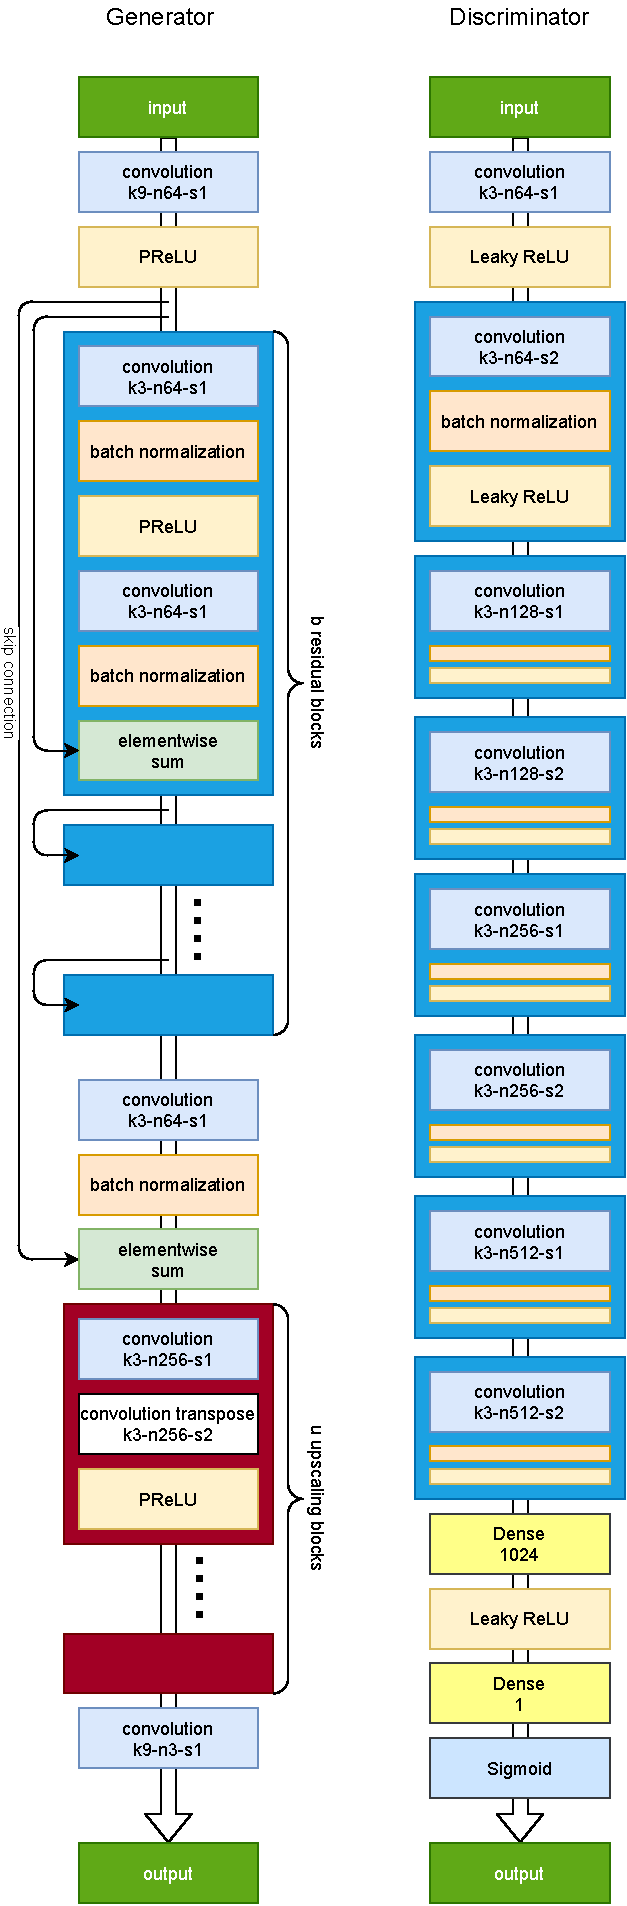
\includegraphics[scale=0.7]{../images/gen_and_dis.pdf}  
        \caption{Generator and Discriminator Network similar to Ledig et al.~\cite{DBLP:journals/corr/LedigTHCATTWS16} }   
        \label{fig:network_architecture}
    \end{figure} 
\end{center}

\subsection{Loss Function}
The loss of the discriminator is defined as $$L_D = L_{fake} + L_{real}$$ where $L_{fake}$ is the binary cross entropy between the discriminator prediction and the ground truth for real images and where $L_{real}$ is the binary cross entropy between the discriminator prediction and the ground truth for fake images.\\
\\
The loss of the generator is defined as $$L_G = L_{G_1} + L_{G_2}$$ where $$L_{G_1}  = {1 \over MN} \sum_{x=1}^M \sum_{y=1}^N (Y_{x,y} - \hat{Y}_{x,y})^2$$ is the pixel-wise Mean Square Error with $Y$ being the original image and $\hat{Y}$ being the generated image. $L_{G_2}$ is the loss of the discriminator.\\
\\
We decided against a more complex approach as described by Ledig et al. \cite{DBLP:journals/corr/LedigTHCATTWS16}, as it seemed to not fit the scope of the project in terms of complexity. However, we expect our results to be better with more sophisticated loss functions.


\section{Experiments}

\subsection{Dataset}
The 2017 Unlabeled images dataset from the Common Objects in Context Dataset (COCO) by Microsoft~\cite{lin2015microsoft} was used as the training dataset. This dataset consists of 123,000 unlabeled images. A dataset of a relatively smaller size has been chosen to minimize the training effort. The images are sourced from 80 object categories. \\
As the dataset consisted of both greyscale and RGB images, all non-RGB images were converted to RGB. This was done via a python script as a one-time operation.


\subsection{Training}
We trained our networks on a NVIDIA RTX 3090 GPU with 24 GB of memory. 
First of all, the paths of the dataset images were read and then shuffled with a large enough buffer size. 
After shuffling, the images were loaded and modified by flipping, cropping, darkening, changing the saturation and brightness with a certain probability. 
Finally, after the images were modified, we create full and low-resolution pairs by resizing the original images. 
We chose the number of upscaling blocks u = 2, which leads to an upscaling factor of $2^{u} = 4$.  
The low-resolution images with the size 64 by 64 pixels are upscaled to full resolution images with the size 256 by 256 pixels.
The optimizer we chose was Adam with ß1 = 0.9, as proposed by Ledig et al.~\cite{DBLP:journals/corr/LedigTHCATTWS16}. 
The learning rate was set to $10^{-4}$, and we trained the network for $10^3$ iterations.
The number of residual blocks was set to b = 8 in order to decrease training effort. 
After encountering a memory problem that leads our GPU's memory usage to increase over time and eventually cause allocation errors, we restructured our training loop and chose to load and save our network after each training iteration. 
After each iteration, one test sample was upscaled by the network to visualize training progress.
This was the only practical way to train the network for a decent number of iterations. 
One training iteration took approximately 800 seconds. The training of 1000 iterations took about 220 hours in total.


\subsection{Inference}
Since the generator network was trained with an input size of 64 by 64 pixels, upscaling larger images is not directly possible.
For this reason, we implemented a program to split images into patches of size 64 by 64, to be able to run them through the generator.
After each patch is scaled up to 256 by 256 pixels, the patches are set back together, resulting in an image that is four times larger then the input. 
Our git repository features a version of the trained network and the script to perform upscaling on any jpg images.

\section*{Discussion}
\subsection{Results}
After 1000 training iterations, the generated images show some of the criteria the upscaling process aims to fulfill.
As seen in figure~\ref{fig:sample_images}, all upscaled images appear a bit more clear and sharp and thus make details easier for the human eye to observe.
In figure~\ref{fig:baby_up}, the nostrils of the baby are way more naturally shaped than in the low resolution image. 
In figure~\ref{fig:butterfly_up}, the patterns on the butterfly's wings are smoothed out. 
Nevertheless, all images are biased towards a specific color and some artifacts show around the edges of the images. 
Furthermore, the edges are sharpened by a fair amount, but this could be improved further.
The problem on the edges gets way more obvious if an image gets scaled up from patches, as seen in figure~\ref{fig:dog_up}. 
At the same time, especially the nose of the dog gets smoothed out and looks subjectively more pleasant.

\begin{figure}[ht] 

\begin{subfigure}{0.45\textwidth}
  \centering
  \begin{minipage}[b]{0.45\textwidth}
    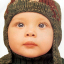
\includegraphics[width=\textwidth]{../images/baby_low.jpg}
    \caption{Baby low}
  \end{minipage}
  \hfill
  \begin{minipage}[b]{0.45\textwidth}
    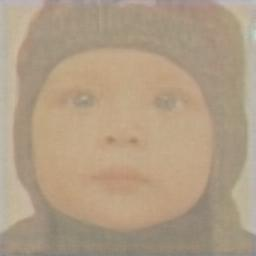
\includegraphics[width=\textwidth]{../images/baby_up.jpg}
    \caption{Baby up}
  \end{minipage}
\end{subfigure}

\par\bigskip

\begin{subfigure}{0.45\textwidth}
  \centering
  \begin{minipage}[b]{0.45\textwidth}
    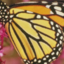
\includegraphics[width=\textwidth]{../images/butterfly_low.jpg}
    \caption{Butterfly low}
  \end{minipage}
  \hfill
  \begin{minipage}[b]{0.45\textwidth}
    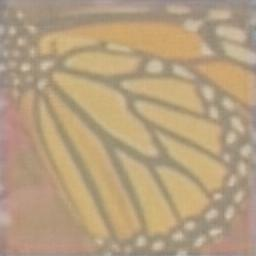
\includegraphics[width=\textwidth]{../images/butterfly_up.jpg}
    \caption{Buttferfly up}
  \end{minipage}
\end{subfigure}

\par\bigskip

\begin{subfigure}{0.45\textwidth}
  \centering
  \begin{minipage}[b]{0.45\textwidth}
    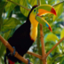
\includegraphics[width=\textwidth]{../images/bird_low.jpg}
    \caption{Bird low}
  \end{minipage}
  \hfill
  \begin{minipage}[b]{0.45\textwidth}
    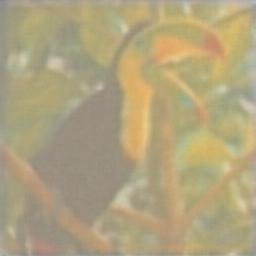
\includegraphics[width=\textwidth]{../images/bird_up.jpg}
    \caption{Bird up}
  \end{minipage}
\end{subfigure}

\par\bigskip

\begin{subfigure}{0.45\textwidth}
  \centering
  \begin{minipage}[b]{0.45\textwidth}
    
\includegraphics[width=\textwidth]{../images/head_low.jpg}
    \caption{Head low}
  \end{minipage}
  \hfill
  \begin{minipage}[b]{0.45\textwidth}
    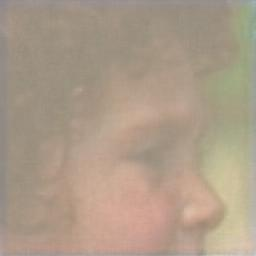
\includegraphics[width=\textwidth]{../images/head_up.jpg}
    \caption{Head up}
  \end{minipage}
\end{subfigure}


\label{fig:sample_images}
\caption{Sample images scaled up by the generator. Images by Bevilacque et al~\cite{BMVC.26.135}}
\end{figure}


\centering
\begin{figure}

    \begin{subfigure}{.12\textwidth}
    \centering
    % include first image
    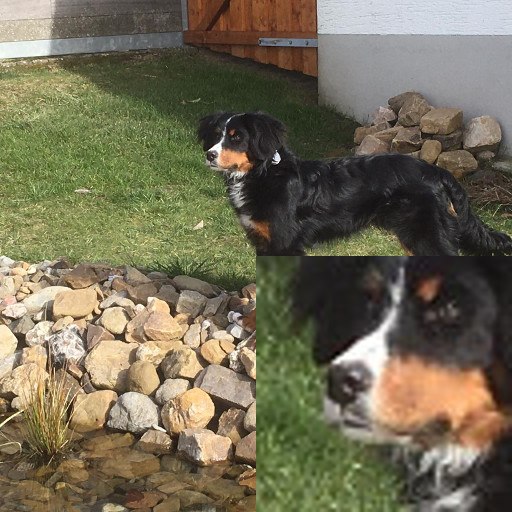
\includegraphics[scale=.5]{../images/dog_low.jpg}  
    \caption{Dog low}
    \label{fig:dog_low}
    \end{subfigure} 
    
    \begin{subfigure}{.12\textwidth}
    \centering 
    % include first image
    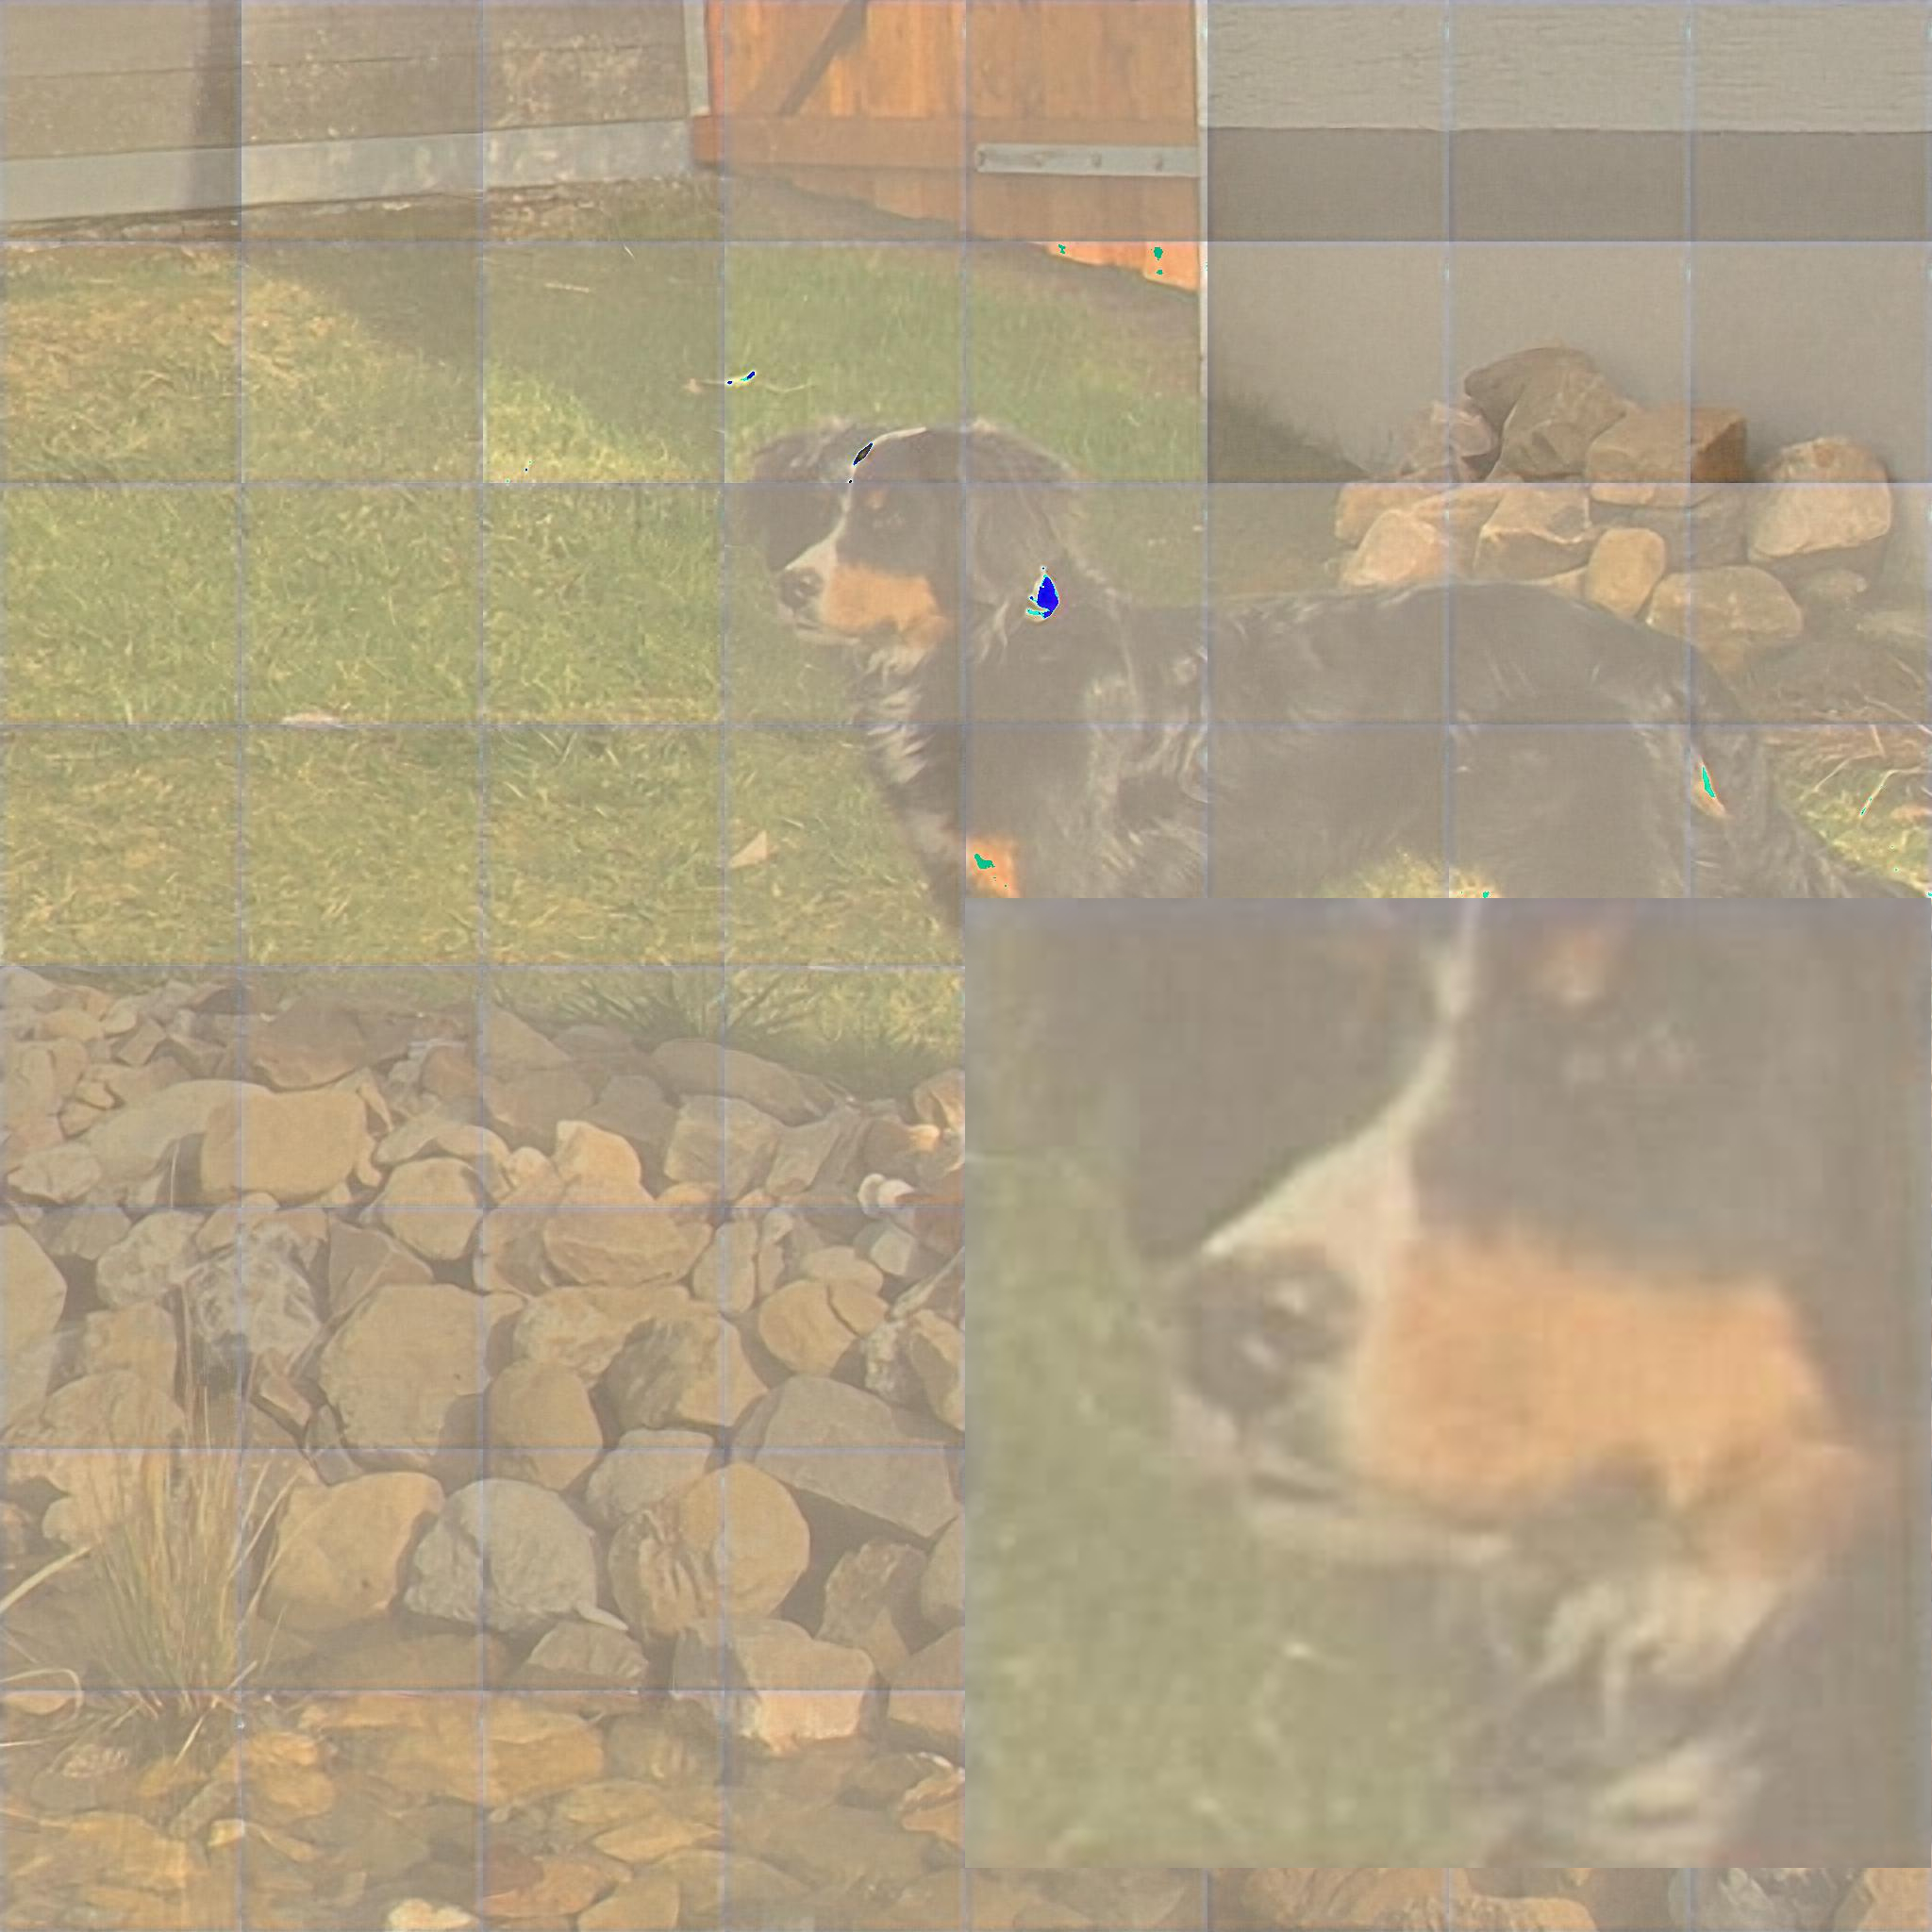
\includegraphics[scale=0.125]{../images/dog_up.jpg}  
    \caption{Dog up}
    \label{fig:dog_up}
    \end{subfigure} 



\label{fig:large_image}
\caption{Large image scaled up in patches.}

    
\end{figure}


\begin{center}
    
\end{center}

\section*{Conclusion}
TODO


\bibliographystyle{ieeetr}
\bibliography{references}

\end{document}
